\chapter{Machine learning}\label{ml_chapter}
    Machine learning is a subfield of artificial intelligence which study systems that learn from data and interactions with the world rather than through explicit programming. The acquired knowledge allows a computer to correctly interpret data that it has never seen before.
    \section{Components of a learning algorithm}\label{components_ml}
        A machine learning algorithm can be built by combining various components, such as an optimization algorithm, a cost function, a model and a dataset.
        \subsection{Dataset}
            The definition of dataset is extremely broad. Basically, a dataset is a collection of data that relates to a particular subject, with the record being the basic unit of information.
            
            Datasets usually are obtained by observing and sampling a statistical population:
            \begin{itemize}
                \item A \emph{record} --- or an example --- corresponds to the observations on one element of that population. The records in a dataset can be organized in various ways.
                \item A \emph{feature} refers to a specific portion of a record --- i.e., a single observation on one element of that population. Features are sometimes referred to as fields.
            \end{itemize}
            Datasets may further be generated by algorithms: this is usually a more inexpensive way to get data.
            
            The value of a feature may be of different types:
            \begin{itemize}
                \item \emph{Nominal data} --- i.e., a feature can take one of a limited, and usually fixed number of possible values. Nominal values lack a numerical meaning, do not have an intrinsic ordering and they can be thought of as labels. A good example is a feature that takes a value from the domain \(\left\{male, female\right\}\).
                \item \emph{Ordinal data} --- i.e., a feature can take one of a limited and ordered number of values. Though the possible values have an intrinsic order, the distance between each one is not really known. For example, a value could be taken from \(\left\{poor, reasonable, good, excellent\right\}\).
                \item \emph{Interval data} --- i.e., a feature can take one number of a numeric scale, where both the order and the differences between the values are known. The Celsius scale is an example.
                \item \emph{Ratio data} --- i.e., a feature can take one number from a domain similar to that of interval data, but where it is also possible to compute ratios of two values. Measuring the weight in kilograms is an example.
            \end{itemize}
            For each feature in different records, the values are normally all of the same kind. However, there may also be missing values, which must be indicated somehow.
        \subsection{Model}
            Machine learning models can be thought of as mathematical models, which aim to explain different components of a system and to make predictions about its behaviour. Models are often a set of relationships between variables --- i.e., abstractions of system parameters --- that can be quantified or described.
            
            Machine learning models usually embody some statistical assumptions about the underlying data-generating process. Specifically, machine learning applications typically assume that there exists an underlying function \(\phi : X \rightarrow Y\) that maps records \(X\) to outcomes \(Y\): a model is a function \(f\) --- chosen from an hypothesis space \(\mathcal{H}\) --- that is assumed to approximate the underlying function \(\phi\) (\(y=\phi\left(x\right)\) and \(\hat{y}=f\left(x\right)\), with \(\hat{y} \approx y\)).
            
            Modelling a system usually implies a trade-off between \emph{flexibility} and \emph{interpretability} of the model \cite[24--26]{James}. On one hand a simple model --- i.e., a model chosen from a restricted hypothesis space --- may be preferred to a complex one when the goal is to understand the relationships between variables and the inferred outcome: when inference is the goal, it is usually better to use simple and relatively inflexible models. On the other hand, in some settings, the goal is to obtain better predictions: a more complex model often increases the accuracy. However, this is not always the case: this phenomenon has to do with the potential of overfitting in highly flexible methods (see section \ref{biasvariance}).
            
            In general, when there are multiple consistent hypotheses to choose from, the simplest one should be preferred over the others: this principle is called Ockham's razor. Defining simplicity is not always easy though.
        \subsection{Cost function}
            Keeping in mind the trade-off between flexibility and interpretability of the model, how can the algorithm choose the function \(f\) that best capture the details of the underlying function \(\phi\)?
            
            Most machine learning problems are defined in terms of cost functions, in the sense that cost functions define what a good model is. Specifically, a cost function --- or loss function --- is a measure of how wrong a model is in terms of its ability to estimate the relationships between different components of a system: if predictions of the model are totally off, the loss function will output a higher number; if they are good, it will output a lower number. Therefore, the objective of a machine learning algorithm is to find a model \(f\) in the hypothesis space \(\mathcal{H}\) that minimizes the cost function \(L\).
            
            Though the cost function is sometimes expressed as the number of wrong classifications, this is not always the case. In general, when the goal is to deduce properties of an underlying probability distribution, different actions or decisions can lead to mistakes, and some of them may be less acceptable than others. A cost function is \textquote{a single overall measure of loss incurred in taking any of the available decisions or actions} \cite[41]{Bishop}.
            
            The choice of a cost function is not a mathematical problem and therefore it cannot be formalized \cite{Hennig}: such choice is an informal and subjective decision. There can't be an objectively best loss function.
        \subsection{Optimization algorithm}
            The optimization algorithm is responsible for actually finding the model \(f\) in the hypothesis space \(\mathcal{H}\) that minimizes the loss function \(L\): choosing an optimization algorithm can make a difference between getting a good accuracy in hours or days. Since a model \(f\) is usually uniquely identified by a vector of parameters \(p\), optimization algorithms find a good model by searching the parameter space.
            
            Optimization algorithms are often iterative procedures: they start from a point \(p^{\left(0\right)}\) --- corresponding to a model \(f^{\left(0\right)}\) in the hypothesis space \(\mathcal{H}\) --- and they generate a sequence of points \(\left\{p^{\left(k\right)}\right\}\): such a sequence will hopefully converges to the global minimum --- i.e., the model \(f \in \mathcal{H}\) that minimizes the loss function \(L\).
            
            It is not easy to classify optimization algorithms because the number of criteria that can be used is high:
            \begin{itemize}
                \item In deterministic optimization algorithms, the output depends entirely on the inputs (and there is a high correlation between the result and the initial point). Instead, stochastic algorithms make use of random variables.
                \item Another criterion is based on the information being used to create new points. First-order optimization algorithms minimize the loss function using its gradient, which indicates the direction of increase/decrease of the function at a particular point. Instead, second-order optimization algorithms use the Hessian matrix, which describes the function's curvature at a particular point.
            \end{itemize}
    \section{Types of learning algorithms}
        \citeauthor{Mitchell} provided a broad definition of machine learning \cite[2]{Mitchell}: \textquote{A computer program is said to learn from experience \(E\) with respect to some class of tasks \(T\) and performance \(P\), if its performance at tasks in \(T\), as measured by \(P\), improves with experience \(E\).}. An algorithm that improves the accuracy of its outputs or predictions over time is said to have learned to perform that task.
        \subsection{Task}
            Machine learning can solve many different tasks that are usually too difficult to solve with algorithms designed by programmers.
            \subsubsection{Classification}\label{classification}
                Classification is the task of identifying which category an example belongs to. Formally, classification algorithms attempt to estimate the mapping function \(f\) from the input features \(X\) to discrete or categorical outputs (outputs are often called labels or categories). In other words, the mapping function predicts the class or category for a given observation. This task can be solved in different ways --- i.e., the function produced by the algorithm can have different goals. For example, a classifier may output one of the following functions:
                \begin{itemize}
                    \item \(f: X \rightarrow C\), mapping examples to a set of categories (\(C = \left\{c_{1}, c_{2}, \dots , c_{k}\right\}\) is the set of possible categories).
                    \item \(f: X \rightarrow \mathcal{K}\left(X_{C}\right)\), mapping examples to discrete probability distributions over classes (\(X_{C}\) is a random variable used to denote the outcome of classification, \(\mathcal{K}\left(X_{C}\right)\) is the set of all discrete probability distributions over classes). It is common in classification tasks to predict the probability of a given input belonging to each output class. The probabilities can be interpreted as the likelihood or confidence of a given example belonging to each class. A predicted probability can be converted into a class value by selecting the class label that has the highest probability.
                \end{itemize}
                Classification becomes even more difficult if it is not guaranteed that every feature will always be provided.
            \subsubsection{Regression}
                Whereas classification is about predicting a label, regression is about predicting a quantity. In this type of task, the machine learning algorithm is asked to predict values of a desired target quantity, where the target quantity is continuous. Formally, regression is the task of approximating a mapping function \(f: X \rightarrow Y\) from the input features \(X\) to a numerical or continuous output variable \(Y\).
        \subsection{Experience}
            A machine learning algorithm is highly influenced by the type of experience available \cite[5]{Mitchell}. According to \citeauthor{Mitchell}, the key attributes of the experience are:
            \begin{itemize}
                \item The type of feedback --- which can be direct or indirect --- regarding the choices made by the algorithm.
                \item The degree to which the learning algorithm controls the sequence of training examples.
                \item How well the provided examples represent the underlying data distribution.
            \end{itemize}
            In the context of the task being addressed --- and depending on the experience available during the learning process --- machine learning algorithms can be classified in different ways. The main classes are those which include unsupervised, supervised and reinforcement learning algorithms. However, there are many more techniques, such as semi-supervised, active and curriculum learning.
            \subsubsection{Unsupervised learning algorithms}
                Unsupervised learning, broadly speaking, involves observing several examples and attempting to implicitly or explicitly find interesting structure in the data. In other words, the agent learns for the sake of learning: unsupervised learning algorithms are designed to create autonomous intelligence and are rewarded for learning about the data they observe without a particular task in mind\footnote{\url{https://deepmind.com/blog/unsupervised-learning/}.}.
                
                More formally, in the unsupervised learning setting, the algorithm has a set of \(n\) observations
                \[x_{1}, x_{2}, \dots, x_{n}\]
                and it tries to learn the probability distribution \(p\left(x\right)\) or some interesting properties of that distribution. 
                
                It can be hard to validate the results of algorithms which learn from such experience, because there is no universally accepted mechanism for checking their answers \cite[374]{James}. In other words, there is no direct measure of success, and one must resort to heuristic arguments for judgments as to the quality of the results \cite[487]{Hastie}.
            \subsubsection{Supervised learning algorithms}\label{supervised}
                Roughly speaking, supervised learning algorithms observe several input-output pairs and learn to predict outputs from inputs. Therefore, such algorithms experience a dataset containing features, but where each example is also associated with a label or target value. The term supervised learning originates from the view of the target being provided by a teacher who shows the learning algorithm what to do \cite[105]{Goodfellow}: under this metaphor, the student provides an answer for each training example, and the supervisor provides either the correct answer or an error associated with the answer \cite[485]{Hastie}. Therefore --- contrary to what happens in unsupervised learning --- with supervised learning there is a clear measure of success that can be used to compare the effectiveness of different methods over various situations \cite[486]{Hastie}.
                
                Formally, given a training set of \(n\) input-output pairs
                \[\left(x_{1},y_{1}\right), \left(x_{2},y_{2}\right), \dots, \left(x_{n},y_{n}\right)\]
                where each \(y_{i}\) was generated by an unknown function \(y=\phi\left(x\right)\) and where \(x\) and \(y\) can be any value (not necessarily numbers), a supervised learning algorithm discovers a function \(f\) in the hypothesis space \(\mathcal{H}\) that approximates the true underlying function \(\phi\). The inferred function can then be used for mapping new examples and determining the class labels of unseen instances.
            \subsubsection{Semi-supervised learning algorithms}\label{semi_supervised}
                In the case of semi-supervised learning algorithms, some of the training examples include a supervision target but others do not: they are halfway between supervised and unsupervised learning algorithms. Typically, these algorithms experience a dataset containing a small amount of labeled data and a large amount of unlabeled data.
                
                Formally, the \(n\) observations can be split in two parts:
                \[\left(x_{1},y_{1}\right), \left(x_{2},y_{2}\right), \dots, \left(x_{l},y_{l}\right)\]
                \[x_{l+1}, x_{l+2}, \dots, x_{n}\]
                where the labels are provided only for \(l\) observations.
                
                Is semi-supervised learning meaningful? \textquote{In comparison with a supervised algorithm that uses only labeled data, can one hope to have a more accurate prediction by taking into account the unlabeled points?} (question arisen by \citeauthor{Chapelle} in \cite[4]{Chapelle}). A number of researchers have found that unlabeled data can considerably improve the learning accuracy. However, there are some prerequisites \cite[4--7]{Chapelle}:
                \begin{itemize}
                    \item The distribution of labeled examples must be relevant for the problem.
                    \item If two points \(x_{1}, x_{2}\) are close, then so should be the corresponding outputs \(y_{1}, y_{2}\) (smoothness assumption).
                    \item if points are in the same cluster, they are likely to be of the same class (cluster assumption).
                    \item The high-dimensional data lie roughly on a low-dimensional manifold (manifold assumption).
                \end{itemize}
                
                Acquiring labeled data is usually very expensive in terms of time, effort or money, since it often requires a person to manually do the work. Therefore, it may be unfeasible to label an entire training dataset: whenever the acquisition of unlabeled data is relatively inexpensive compared to that of labeled data, semi-supervised learning can be helpful. Notice, though, that in general unlabeled data carry less information than labeled data, and thus they are required in large amounts.
            \subsubsection{Reinforcement learning algorithms}
                In a reinforcement learning setting, an agent is asked to learn how to behave in a dynamic environment through trial-and-error interactions \cite{Kaelbling}: in other words, there is a feedback loop between the learning algorithm and its experiences.
                
                A reinforcement learning algorithm does not experience a fixed dataset. Instead, after choosing an action the agent is given a reward and is told the subsequent state: in order to act optimally, the agent must actively gather experience about the possible states, actions, transitions and reward (online experience).
            \subsubsection{Active learning algorithms}\label{active_learning}
                In a supervised learning setting, many labeled examples are often required if one wants to achieve a high accuracy. Moreover, there are situations in which it is very time-consuming, difficult or expensive to obtain such an amount of labels, even though unlabeled data is abundant \cite[4]{Settles}. Here are a couple of examples:
                \begin{itemize}
                    \item Annotating an audio file at the word level (or at the phonemes one) takes an extremely long time compared to the length of the audio file. Also, a specialized and trained linguist is often required.
                    \item Classifying web pages or images does not take a long time but it can be very redundant, and therefore subject to error.
                \end{itemize}
                
                In an active learning setting, a learning algorithm can achieve greater performance with less data if it is allowed to obtain the examples it desires and from which it learns. In other words, the cost of obtaining data is minimized by allowing the algorithm to decide which instances should be labeled in order to achieve a high accuracy.
                
                Active learning algorithms are able to query an information source --- or oracle --- to get the desired inputs, thus decreasing the risk of being overwhelmed by useless examples --- i.e., inputs which do not carry useful information. A diagram of how active learning works is shown in figure \ref{active_learning_cycle}.
                
                \begin{figure}
    \centering
    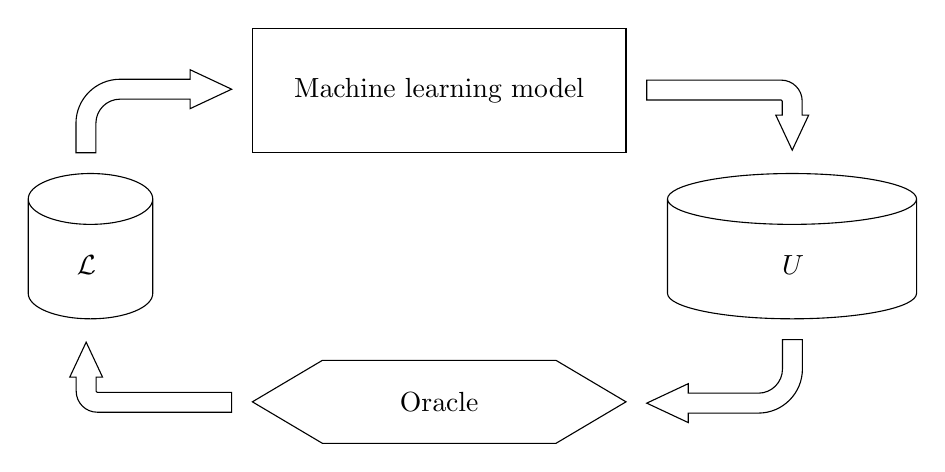
\begin{tikzpicture}[x=0.75pt,y=0.75pt,yscale=-1,xscale=1]
        %Flowchart: Magnetic Disk [id:dp9287936135344942] 
        \draw   (82,122.25) -- (82,167.75) .. controls (82,174.52) and (68.57,180) .. (52,180) .. controls (35.43,180) and (22,174.52) .. (22,167.75) -- (22,122.25)(82,122.25) .. controls (82,129.02) and (68.57,134.5) .. (52,134.5) .. controls (35.43,134.5) and (22,129.02) .. (22,122.25) .. controls (22,115.48) and (35.43,110) .. (52,110) .. controls (68.57,110) and (82,115.48) .. (82,122.25) -- cycle ;
        %Flowchart: Magnetic Disk [id:dp374407561883777] 
        \draw   (450,122.25) -- (450,167.75) .. controls (450,174.52) and (423.14,180) .. (390,180) .. controls (356.86,180) and (330,174.52) .. (330,167.75) -- (330,122.25)(450,122.25) .. controls (450,129.02) and (423.14,134.5) .. (390,134.5) .. controls (356.86,134.5) and (330,129.02) .. (330,122.25) .. controls (330,115.48) and (356.86,110) .. (390,110) .. controls (423.14,110) and (450,115.48) .. (450,122.25) -- cycle ;
        %Flowchart: Preparation [id:dp06966809995247569] 
        \draw   (130,220) -- (163.75,200) -- (276.25,200) -- (310,220) -- (276.25,240) -- (163.75,240) -- cycle ;
        %Bend Arrow [id:dp5182616743082409] 
        \draw   (395,190) -- (395,204.17) .. controls (395,215.91) and (385.48,225.43) .. (373.75,225.43) -- (340,225.43) -- (340,230) -- (320,220.63) -- (340,211.25) -- (340,215.83) -- (373.75,215.83) .. controls (380.18,215.83) and (385.4,210.61) .. (385.4,204.17) -- (385.4,190) -- cycle ;
        %Bend Arrow [id:dp8578173985872724] 
        \draw   (120,225) -- (55.24,225) .. controls (49.65,225) and (45.11,220.47) .. (45.11,214.88) -- (45.11,208.13) -- (42,208.13) -- (49.91,191.25) -- (57.82,208.13) -- (54.71,208.13) -- (54.71,214.88) .. controls (54.71,215.17) and (54.94,215.41) .. (55.24,215.41) -- (120,215.41) -- cycle ;
        %Flowchart: Process [id:dp753078500376894] 
        \draw   (130,40) -- (310,40) -- (310,100) -- (130,100) -- cycle ;
        %Bend Arrow [id:dp18815347737102261] 
        \draw   (45,100) -- (45,85.83) .. controls (45,74.09) and (54.52,64.58) .. (66.26,64.58) -- (100,64.58) -- (100,60) -- (120,69.38) -- (100,78.75) -- (100,74.17) -- (66.26,74.17) .. controls (59.82,74.17) and (54.6,79.39) .. (54.6,85.83) -- (54.6,100) -- cycle ;
        %Bend Arrow [id:dp0737210580323302] 
        \draw   (320,65) -- (384.76,65) .. controls (390.35,65) and (394.89,69.53) .. (394.89,75.13) -- (394.89,81.88) -- (398,81.88) -- (390.09,98.75) -- (382.18,81.88) -- (385.29,81.88) -- (385.29,75.13) .. controls (385.29,74.83) and (385.06,74.59) .. (384.76,74.59) -- (320,74.59) -- cycle ;
        
        % Text Node
        \draw (50,154) node   {$\mathcal{L}$};
        % Text Node
        \draw (390.5,154) node   {$U$};
        % Text Node
        \draw (220,220) node  [align=left] {Oracle};
        % Text Node
        \draw (220,70) node  [align=left] {Machine learning model};
    \end{tikzpicture}
    \caption{The active learning cycle. At the beginning, only a small number of labeled instances can be used by the learner (labeled training set \(\mathcal{L}\): the learner proceeds in a standard (semi-)supervised way, building a model starting from \(\mathcal{L}\). Then, the algorithm can query an oracle requesting labels for a number of examples: usually, there is a huge amount of unlabeled examples to choose from --- i.e., the unlabeled training set \(\mathcal{U}\). The new labeled instances are added to the set \(\mathcal{L}\), and the cycle starts again.}
    \label{active_learning_cycle}
\end{figure}
                
                Clearly, when designing an active learning algorithm one must define what is the query strategy: how to decide which instances are most informative and thus more desirable than others? Many strategies have been proposed, and here are a few examples:
                \begin{itemize}
                    \item A query system may label instances which are likely to be updated with the greatest magnitude --- i.e., it may label those instances that are most different from the current model. While this strategy is simple and fast, unrepresentative regions of the space may be found, thus introducing noise in the model.
                    \item Query-by-Committee approaches select examples in which disagreement among multiple classifiers is high. In other words, the utility of an example is measured in terms of disagreement in the committee about its predicted label.
                    \item Some query systems try to reduce the expected error reduction, labelling those points that would most reduce the model's generalization error. These methods are able to optimize the performance of the model, but at the same time they are very expensive and it is usually not possible to compute all unlabelled data.
                    \item The query systems based on representativeness label instances that can represent the underlying distribution of training instances.
                \end{itemize}
                
                Active learning is closely related to semi-supervised learning since both of them aim at making the most out of unlabeled data. However, they attack the same problem from opposite directions: \textquote{while semi-supervised methods exploit what the learner thinks it knows about the unlabeled data, active methods attempt to explore the unknown aspects} \cite[45]{Settles}. Therefore, it may be a good idea to combine these two approaches.
            \subsubsection{Curriculum learning algorithms}\label{cv_learning}
                In \citeyear{Bengio}, \citeauthor{Bengio} presented a novel approach called curriculum learning \cite{Bengio}: it is a type of learning in which at first the algorithm is presented simple examples, and then the difficulty of the tasks it has to solve gradually increases. Citing the authors of the paper, \textquote{by choosing which examples to present and in which order to present them to the learning system, one can guide training and remarkably increase the speed at which learning can occur} --- i.e., instances are somehow sorted and then presented to the algorithm in that specific order, rather than using a random approach. In other words, the training set is imposed a structure.
                
                The ideas behind curriculum learning come from the way in which humans and animals seem to learn better. In the education system, for example, children learn according to this principle: they start small --- i.e., they first start out with only simple tasks --- and gradually increase the difficulty level of the concepts they study. Being introduced to concepts by increasing complexity allows the learner to use previous experience to ease the learning of new concepts.
                
                Defining the curriculum is not an easy task, and general principles that make some strategies work better than others are still unknown. In general, there are two problems that must be solved \cite{Hacohen}:
                \begin{itemize}
                    \item What are the notions of \textquote{easy} and \textquote{hard} instances? Indeed, in order to impose the training set a structure, one must sort the examples by complexity, and it is not always easy to define when an instance is easier than another one. For example, in some settings an hard concept may be an ambiguous one (teachers tend to present typical examples first, followed by more ambiguous ones).
                    \item How much time should the learner spend on each difficulty level? Going over the concepts too fast or too slowly may lead to unproductive learning. Also, how many examples should be presented to the learner at each phase? Learning may be unproductive if an algorithm which does not have enough past experience is overwhelmed by difficult information.
                \end{itemize}
                
                In general, it is faster to train a model in a curriculum learning setting since the learner does not try to learn difficult concepts when it is not ready --- i.e., without having enough past experience. In other words, the learner does not waste time with noisy or harder to predict examples when it is not ready to do it \cite{Bengio}. More importantly, curriculum learning is likely to speed up the convergence of the optimization algorithm --- i.e., it guides it towards better local minima.
    \section{Generalizability of a learned model}\label{generalizability}
        A machine learning model must perform well on new, previously unseen inputs, so that it can make accurate predictions. In other words, a good model would perform in a \textquote{reasonable} way when dealing with previously unseen data. Generalization refers to the ability to perform effectively on previously unobserved data --- i.e., predicting accurate outcome values on examples the algorithm was not trained on.
        \subsection{Generalization error}
            The generalization error measures how likely the model is to make an error. In other words, it is the expected value of the error on a new input \cite[12]{Mohri}.
            
            Formally, given a model \(f \in \mathcal{H}\), the true function \(\phi\), and the underlying distribution \(\mathcal{D}\), the generalization error of \(f\) is defined by
            \[GE\left(f\right) = \underset{x \sim \mathcal{D}}{Pr}\left(f\left(x\right) \ne \phi\left(x\right)\right)\]
            
            Most of the times, the generalization error is not known since both the underlying distribution \(\mathcal{D}\) and the true function \(\phi\) are not accessible. Therefore, one must estimate the generalization error of a machine learning model: this can be done by calculating the empirical error, which measures the model's performance on a test set of examples that were collected separately from the training set.
            
            Formally, given a test set \(\left\{\left(x_{1},y_{1}\right), \left(x_{2},y_{2}\right), \dots, \left(x_{n},y_{n}\right)\right\}\) and a model \(f \in \mathcal{H}\), the empirical error of \(f\) is defined by
            \[\widehat{GE}\left(f\right) = \frac{1}{n}\sum_{i=1}^{n}1_{f\left(x_{i}\right) \ne y_{i}}\]
            
            To sum up, the empirical error of \(f\in\mathcal{H}\) is its average error over the test set, while the generalization error is its expected error based on the distribution \(\mathcal{D}\). Under certain assumptions, it is true that \(GE \approx \widehat{GE}\). Specifically, one must assume that \cite[111]{Goodfellow}:
            \begin{itemize}
                \item The training set --- i.e., the examples used to find the best \(f\in\mathcal{H}\) --- and the test set --- i.e., the examples used to measure the empirical error --- are identically distributed, that is they are generated by the same probability distribution.
                \item The examples in each dataset are independent from each other.
            \end{itemize}
            The higher the quality of data --- i.e., the more they are representative of the underlying distribution \(\mathcal{D}\) --- the easier it will be for the model to successfully learn the true function \(f\) mapping inputs to outputs.
        \subsection{Bias and variance}\label{biasvariance}
            The term bias refers to the systematic error that the learning algorithm is expected to make for a given number of examples. In other words, it measures how far the predicted values are from the actual values. 
            
            Formally, suppose to repeatedly draw training samples \(S_{1},S_{2},\dots,S_{l}\), each of size \(m\), and construct models \(f_{S_{1}},f_{S_{2}},\dots,f_{S_{l}}\) by applying the learning algorithm A. These models can be combined into an average model:
            \[\bar{f}\left(x\right) = \lim_{l \rightarrow \infty}\frac{1}{l}\sum_{i=1}^{l}f_{S_{i}}\left(x\right)\]
            The value \(\bar{f}\left(x\right)\) is the expected predicted value of \(f\left(x\right)\), where the expectation is taken over all possible training samples of size \(m\). The bias of algorithm \(A\) for sample size \(m\) at point \(x\) is the error in this average model:
            \[Bias\left(A,m,x\right) = \bar{f}\left(x\right) - f\left(x\right)\]
            
            A concept strictly related to bias is variance. It captures how much the algorithm's predictions are spread out from their average value.
            
            Formally, the variance of an algorithm is defined as
            \[Variance\left(A,m,x\right) = E\left[\left(f_{S} - \bar{f}\left(x\right)\right)^{2}\right]\]
            where the expectation is taken with respect to all training samples \(S\) of size \(m\).
            
            It is very important to design a learning algorithm that simultaneously minimized bias and variance, since the empirical error \(\widehat{GE}\left(f\right)\) depends on both of them. For example, in \cite{Geman} \citeauthor{Geman} have shown that if one measure the generalization error by using \(E\left[\left(\phi\left(x\right) - f\left(x\right)\right)^2 \mid \mathcal{D}\right]\) --- i.e., the mean squared error with respect to the underlying probability distribution \(\mathcal{D}\) --- then the generalization error can be decomposed as follows:
            \[Bias^2\left(A,m,x\right) + Variance\left(A,m,x\right) + irreducible\ error\]
            
            Bias and variance correspond to two important issues in machine learning: underfitting and overfitting:
            \begin{itemize}
                \item Underfitting occurs when a model obtains a high error value on the training set, and the generalization error estimated on the test set is very similar to that error. Such a model usually has high bias and low variance, and it is unable to capture the complex patterns in the data.
                \item Overfitting occurs when the gap between the training error and the generalization error estimated on the test set is too large. Such a model usually has low bias and high variance, and it is too dependent on the data.
            \end{itemize}
            There are many ways in which it is possible to control whether a model is more likely to overfit or underfit. For example, this can be done by controlling its representational capacity \cite[111-113]{Goodfellow} --- i.e., the ability to fit a wide variety of functions: while models with insufficient capacity cannot solve complex tasks, those with a too high capacity may overfit.
            
            Another technique for controlling a model's capacity is expressing preferences for one function over another: this is a more general way than including or excluding a function from a hypothesis space. More details can be found in section \ref{regularization}.
        \subsection{No free lunch theorem}
            The no free lunch theorem for machine learning \cite{Wolpert} states that every learning algorithm has the same average performance if run over all possible data generating distributions. In other words, there is no model that works best for every task. Intuitively, it is not possible to find a model that is able to infer a rule describing every member of a set, given only information about a subset of examples.
            
            However, these results hold only when the algorithm's predictions are averaged over all possible data generating distributions. In fact, it is possible to apply machine learning algorithms as long as some assumptions about the data probability distribution hold. 
            
            The no free lunch theorem implies that machine learning algorithms must be designed to perform a specific task. They can generalize to previously unseen data by providing probabilistic rules rather than logical rules: the goal is to find a model that is likely to provide the right answer for most of the examples --- not to seek a universal learning algorithm that is able to work on data drawn from all distributions.
        \subsection{Regularization}\label{regularization}
            Roughly speaking, regularization is a technique for giving a preference for one solution in the hypothesis space \(\mathcal{H}\) to another. The other solution will be chosen only if its performance are significantly better than that of the preferred solution. In other words, \textquote{regularization is any modification we make to a learning algorithm that is intended to reduce its generalization error but not its training error} \cite[120]{Goodfellow}.
            
            Regularization helps learning algorithms in exploring certain regions of the hypothesis space \(\mathcal{H}\) and is useful for preventing overfitting. More generally, it can be used for improving the generalizability of a learned model.
            
            There are many ways in which preferences can be expressed:
            \begin{itemize}
                \item A simple one consists in adding a penalty term \(R\left(f\right)\) --- or regularizer --- to the loss function \(L\):
                \[L\left(\hat{y}_{i},y_{i}\right) + \lambda R\left(f\right)\]
                where \(\lambda\) is a parameter that controls the importance of the regularizer. In the so-call weight decay technique\footnote{The weight decay technique is also known as ridge regression in statistics. In mathematics, it is known as Tikhonov regularization.}, \(R\left(f\right) = \left\Vert\Gamma x\right\Vert_{2}^{2}\), where \(\left\Vert\cdot\right\Vert_{2}\) is the Euclidean norm and \(\Gamma\) is the Tikhonov matrix\footnote{In many cases, the Tikhonov matrix is chosen as a multiple of the identity matrix (\(\Gamma + \alpha I\)).}.
                \item Early stopping is an implicit regularization technique used when the model is trained by an iterative optimization algorithm. It consists in stopping the training of a model when certain conditions hold (for example, the accuracy may be under a threshold). Intuitively, an iterative procedure will learn more and more complex models as it run: by regularizing on time, the flexibility of the model can be controlled.
            \end{itemize}
    \section{Model selection and assessment}
        Assessing the generalization performance of a learning algorithm --- i.e., its prediction capability on an independent test set --- is very important, since it helps to choose the best model and measures the quality of the ultimately chosen model \cite[219]{Hastie}.
        
        There are two different goals that one may want to achieve:
        \begin{description}
            \item[Model selection] Selecting the best model from a set of competing candidates. This can be done by estimating the performance of different models using available data. It is not always clear what is meant by best: a good model should balance efficiency with simplicity.
            \item[Model assessment] Estimating the prediction error on new unseen data. This can be done once the final model has been chosen. The measure obtained can be used as an estimator of the true error of the learned model.
        \end{description}
        If there are many data, the best technique for achieving both goals is to use a subset of the dataset. However, in order to have an honest evaluation of the generalization performance, the test set used for assessing the final model should be always used only at the end of the data analysis: using it during model training or selection would make the test error underestimates the generalization error of the final chosen model.
        \subsection{Performance measure}
            Choosing the metrics to evaluate, measure and compare the learned model --- and, in general, the learning algorithm --- is a very important step, since this choice will influence future actions. 
            
            These performance metrics should not be confused with the cost function used to train the model \cite[423]{Goodfellow}: while the cost function is minimized by the optimization algorithm to optimize the model, the metric is used to judge the performance of the model and has nothing to do with the optimization process. In fact, many performance metrics cannot be easily optimized since they are not smooth or single-value.
            
            There are many different performance metrics that can be used to measure the effectiveness of a complete machine learning application.
            \subsubsection{Regression metrics}
                There exist many performance metrics used for evaluating regression algorithms (in a supervised learning setting). Some of the most popular ones are mean square error and root mean square error.
                
                Formally, given an evaluation set \(\left\{\left(x_{1},y_{1}\right), \left(x_{2},y_{2}\right), \dots, \left(x_{n},y_{n}\right)\right\}\) of \(n\) input-output pairs, where each \(y_{i}\) was generated by an unknown function \(y=\phi\left(x\right)\), and given a function \(f \in \mathcal{H}\) found by the learning algorithm, the metrics are defined as follows:
                \[MSE = \frac{1}{n}\sum_{i=1}^{n}\left(f\left(x_{i}\right) - y_{i}\right)^{2} \quad RMSE = \sqrt{\frac{1}{n}\sum_{i=1}^{n}\left(f\left(x_{i}\right) - y_{i}\right)^{2}}\]
                
                Another widely used metric for regression is the coefficient of determination. It is a statistical measure of how well the regression predictions approximate the real data points:
                \[R^{2} = 1 - \frac{\sum_{i=1}^{n}\left(f\left(x_{i}\right) - y_{i}\right)^{2}}{\sum_{i=1}^{n}\left(f\left(x_{i}\right) - \bar{y}\right)^{2}}\]
                where \(\bar{y} = \frac{1}{n}\sum_{i=1}^{n}y_{i}\) is the mean of the \(n\) examples in the evaluation set. An \(R^{2}\) of 1 indicates that the regression predictions perfectly fit the data.
            \subsubsection{Clustering metrics}
                It is more difficult to evaluate an unsupervised learning algorithm, since there is no ground truth when dealing with unlabeled data. However, even though there are no ways to directly measure the quality of model's predictions, there are some heuristic metrics that can give useful insights into how data might change depending on the choice of the algorithm.
                
                Here are some of the most famous examples of metrics used for evaluating clustering algorithms:
                \begin{itemize}
                    \item The Davies-Bouldin index measures if clusters are well-spaced from each other and how much dense they are.
                    \item The silhouette coefficient measures how similar an example is to its own cluster compared to other clusters.
                \end{itemize}
            \subsubsection{Classification metrics}
                There are two tasks in which classification can fall: binary --- i.e., the input has to be classified into one of two non-overlapping classes --- or multi-class --- i.e., the input has to be classified into one of \(K\) classes. There exists a number of metrics that can be used in both cases \cite{Sokolova}.
                
                Assessing the quality of classification can be done by using a confusion matrix and counting the number of correctly or mistakenly labeled examples. Confusion matrix is an easy metric for assessing the correctness of a classification model. It can be represented as a square table, where one axis represents the label that the model predicted, and the other axis is the actual label. See table \ref{confusion_matrix} for an example of a confusion matrix for a binary classification problem.
                
                \begin{table}
                    \centering
                    \renewcommand{\arraystretch}{2}
                    \begin{tabular}{l|l|c|c|}
                        \multicolumn{2}{c}{} & \multicolumn{2}{c}{Actual label}\\
                        \cline{3-4}
                        \multicolumn{2}{c|}{}&Positive&Negative\\
                        \cline{2-4}
                        \multirow{2}{*}{Predicted label}& Positive & TP & FP\\
                        \cline{2-4}
                        & Negative & FN & TN \\
                        \cline{2-4}
                    \end{tabular}
                    \caption{The confusion matrix for a binary classification problem is a \(2 \times 2\) table that reports the number of true positives, false positives, false negatives and true negatives --- i.e., TP, FP, FN and TN. If the model correctly predicts the positive class then the outcome is a true positive. Similarly, true negatives count how many times the model correctly predicts the negative class. A false positive is an outcome in which the model mistakenly predicted the positive class. Finally, a false negative is an outcome where the model incorrectly predicts the negative class.}
                    \label{confusion_matrix}
                \end{table}
                
                The main performance metrics used for binary classifications are the following:
                \begin{itemize}
                    \item Accuracy evaluates the overall performance of a classifier by measuring the fraction of predictions the model got right.
                    \item Precision measures the fraction of results which are relevant.
                    \item Recall refers to the fraction of total relevant results correctly classified by the model.
                    \item F\textsubscript{1} score measures the relations between data’s positive labels and those given by the classifier.
                \end{itemize}
                Definitions of these performance metrics are summarized in table \ref{binary_metrics}.
                
                \begin{table}
                    \centering
                    \renewcommand{\arraystretch}{2}
                    \begin{tabulary}{\textwidth}{|C|C|}
                        \hline
                        Measure & Formula \\ \hline \hline
                        Accuracy & \(\frac{TP+TN}{TP+FN+FP+TN}\) \\ \hline
                        Precision & \(\frac{TP}{TP+FP}\) \\ \hline
                        Recall & \(\frac{TP}{TP+FN}\) \\ \hline
                        F\textsubscript{1} score & \(\frac{\left(\beta^{2}+1\right) \cdot TP}{\left(\beta^{2}+1\right)\cdot TP+\beta^{2}\cdot FN+FP}\) \\ \hline
                    \end{tabulary}
                    \caption{Definitions of performance metrics for binary classification (using the notation introduced in table \ref{confusion_matrix}).}
                    \label{binary_metrics}
                \end{table}
                
                Performance metrics used for binary classification can be extended to the multi-class setting \cite{Sokolova}. Specifically, given a class \(C_{i}\), the assessment can be done using \(TP_i\), \(FN_i\), \(TN_i\) and \(FP_i\) --- i.e., the values of the confusion matrix from the counts for \(C_i\).
                
                In many cases, a single value that summarizes the performance of the classifier is desirable. Quality of overall classification is assessed either using macro-averaging or micro-averaging:
                \begin{itemize}
                    \item Macro-averaging means taking the average of a single metric measured independently on different classes.
                    \item In Micro-averaging the individual values for different classes are aggregated and then combined to get the desired metric.
                \end{itemize}
                In a multi-class setting, micro-average is preferable if there might be class imbalance --- i.e., many more examples of one class than of other classes.
                
                Definitions of performance metrics used for a multi-class setting are summarized in table \ref{multiclass_metrics}.
                
                \begin{table}
                    \centering
                    \renewcommand{\arraystretch}{2.5}
                    \begin{tabulary}{\textwidth}{|C|C|}
                        \hline
                        Measure & Formula \\ \hline \hline
                        Average accuracy & \(\frac{1}{K}\sum_{i=1}^{K}\frac{TP_i+TN_i}{TP_i+FN_i+FP_i+TN_i}\) \\ \hline
                        Precision\textsubscript{\(M\)} & \(\frac{1}{K}\sum_{i=1}^{K}\frac{TP_i}{TP_i+FP_i}\) \\ \hline
                        Precision\textsubscript{\(\mu\)} & \(\frac{\sum_{i=1}^{K}TP_i}{\sum_{i=1}^{K}\left(TP_i+FP_i\right)}\) \\ \hline
                        Recall\textsubscript{\(M\)} & \(\frac{1}{K}\sum_{i=1}^{K}\frac{TP_i}{TP_i+FN_i}\) \\ \hline
                        Recall\textsubscript{\(\mu\)} & \(\frac{\sum_{i=1}^{K}TP_i}{\sum_{i=1}^{K}\left(TP_i+FN_i\right)}\) \\ \hline
                        F\textsubscript{1} score\textsubscript{\(M\)} & \(\frac{\left(\beta^2+1\right) \cdot Precision_M \cdot Recall_M}{\beta^2 \cdot Precision_M + Recall_M}\) \\ \hline
                        F\textsubscript{1} score\textsubscript{\(\mu\)} & \(\frac{\left(\beta^2+1\right) \cdot Precision_{\mu} \cdot Recall_{\mu}}{\beta^2 \cdot Precision_{\mu} + Recall_{\mu}}\) \\ \hline
                    \end{tabulary}
                    \caption{Definitions of performance metrics for multi-class classification. \(M\) and \(\mu\) indices represent macro-averaging and micro-averaging respectively.}
                    \label{multiclass_metrics}
                \end{table}
        \subsection{Validation}\label{validation}
            There is a variety of model selection methods, and validation is one of them. Basically, the available dataset is split in two parts: one is used to train candidate models, and the other for deciding which is better \cite[145]{Shalev-Shwartz}.
            \subsubsection{Validating using hold-out samples}
                The simplest approach to validation is using an hold-out sample. A hold-out sample --- or validation dataset --- is a separate dataset used for selecting models: while the training dataset is used for fitting and finding new candidate models, the hold-out dataset can be used for comparing the performance of multiple models and for choosing the best one in an unbiased way.
                
                This method is very simple: it is good to use when the dataset is very large and, in general, when other approaches may take too long.
            \subsubsection{Validating using \(k\)-fold cross-validation}
                When there are few data --- and it is not possible to \textquote{waste} data on validation --- \(k\)-fold cross-validation may be a good choice.
                
                In \(k\)-fold cross-validation the dataset is split into \(k\) roughly equal-sized subsets --- or folds. A model is trained on the union of \(k-1\) subsets, and then the error is estimated using the remaining fold. This is repeated for each subset. Finally, all the errors are averaged, obtaining an estimate of the true error, which can be used to compare different models and choose the best one.

                Cross-validation is usually preferred over the hold-out technique. Indeed, while hold-out is strictly dependent on how the dataset was split, cross-validation gives a very good indication of how well the model will perform on unseen data. This is due to the fact that the model is trained multiple times on train-validation splits. However, the computational burden of \(k\)-fold cross-validation is also considerable: this technique requires much more computational power and time to run compared to hold-out. Therefore, a trade-off might be required.
                
                \begin{figure}
    \centering
    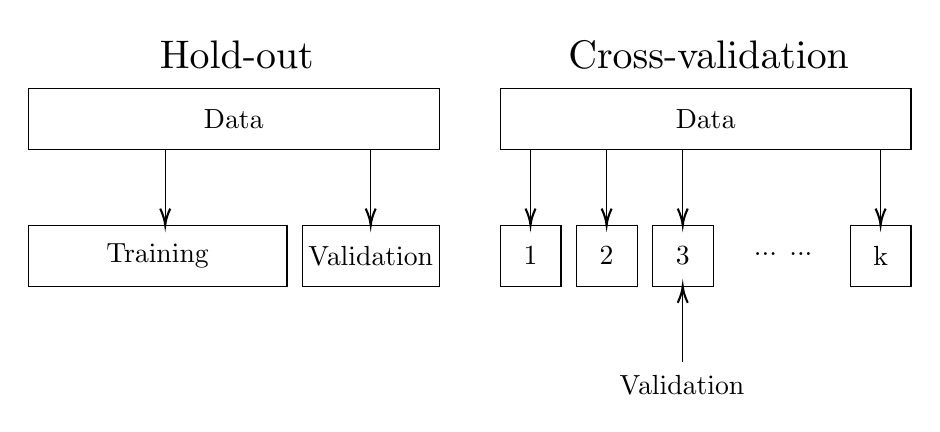
\begin{tikzpicture}[x=0.55pt,y=0.55pt,yscale=-1,xscale=1]
        %Shape: Rectangle [id:dp30782299997247864] 
        \draw   (30,40) -- (300,40) -- (300,80) -- (30,80) -- cycle ;
        %Shape: Rectangle [id:dp5159914550919137] 
        \draw   (340,40) -- (610,40) -- (610,80) -- (340,80) -- cycle ;
        %Shape: Rectangle [id:dp8069194161926109] 
        \draw   (30,130) -- (200,130) -- (200,170) -- (30,170) -- cycle ;
        %Shape: Rectangle [id:dp959684597440048] 
        \draw   (210,130) -- (300,130) -- (300,170) -- (210,170) -- cycle ;
        %Shape: Rectangle [id:dp8001671544362841] 
        \draw   (340,130) -- (380,130) -- (380,170) -- (340,170) -- cycle ;
        %Shape: Rectangle [id:dp19700561762726387] 
        \draw   (570,130) -- (610,130) -- (610,170) -- (570,170) -- cycle ;
        %Shape: Rectangle [id:dp6964850406597634] 
        \draw   (390,130) -- (430,130) -- (430,170) -- (390,170) -- cycle ;
        %Shape: Rectangle [id:dp5278376415103712] 
        \draw   (440,130) -- (480,130) -- (480,170) -- (440,170) -- cycle ;
        %Straight Lines [id:da17033992216894744] 
        \draw    (360,80) -- (360,128) ;
        \draw [shift={(360,130)}, rotate = 270] [color={rgb, 255:red, 0; green, 0; blue, 0 }  ][line width=0.75]    (10.93,-3.29) .. controls (6.95,-1.4) and (3.31,-0.3) .. (0,0) .. controls (3.31,0.3) and (6.95,1.4) .. (10.93,3.29)   ;
        
        %Straight Lines [id:da5076595148790187] 
        \draw    (410,80) -- (410,128) ;
        \draw [shift={(410,130)}, rotate = 270] [color={rgb, 255:red, 0; green, 0; blue, 0 }  ][line width=0.75]    (10.93,-3.29) .. controls (6.95,-1.4) and (3.31,-0.3) .. (0,0) .. controls (3.31,0.3) and (6.95,1.4) .. (10.93,3.29)   ;
        
        %Straight Lines [id:da6592490936454037] 
        \draw    (460,80) -- (460,128) ;
        \draw [shift={(460,130)}, rotate = 270] [color={rgb, 255:red, 0; green, 0; blue, 0 }  ][line width=0.75]    (10.93,-3.29) .. controls (6.95,-1.4) and (3.31,-0.3) .. (0,0) .. controls (3.31,0.3) and (6.95,1.4) .. (10.93,3.29)   ;
        
        %Straight Lines [id:da8377856383779624] 
        \draw    (590,80) -- (590,128) ;
        \draw [shift={(590,130)}, rotate = 270] [color={rgb, 255:red, 0; green, 0; blue, 0 }  ][line width=0.75]    (10.93,-3.29) .. controls (6.95,-1.4) and (3.31,-0.3) .. (0,0) .. controls (3.31,0.3) and (6.95,1.4) .. (10.93,3.29)   ;
        
        %Straight Lines [id:da5318453015444125] 
        \draw    (120,80) -- (120,128) ;
        \draw [shift={(120,130)}, rotate = 270] [color={rgb, 255:red, 0; green, 0; blue, 0 }  ][line width=0.75]    (10.93,-3.29) .. controls (6.95,-1.4) and (3.31,-0.3) .. (0,0) .. controls (3.31,0.3) and (6.95,1.4) .. (10.93,3.29)   ;
        
        %Straight Lines [id:da5175740274992974] 
        \draw    (255,80) -- (255,128) ;
        \draw [shift={(255,130)}, rotate = 270] [color={rgb, 255:red, 0; green, 0; blue, 0 }  ][line width=0.75]    (10.93,-3.29) .. controls (6.95,-1.4) and (3.31,-0.3) .. (0,0) .. controls (3.31,0.3) and (6.95,1.4) .. (10.93,3.29)   ;
        
        %Straight Lines [id:da7508158168507306] 
        \draw    (460,172) -- (460,220) ;
        
        \draw [shift={(460,170)}, rotate = 90] [color={rgb, 255:red, 0; green, 0; blue, 0 }  ][line width=0.75]    (10.93,-3.29) .. controls (6.95,-1.4) and (3.31,-0.3) .. (0,0) .. controls (3.31,0.3) and (6.95,1.4) .. (10.93,3.29)   ;
        
        % Text Node
        \draw (255,150) node  [align=left] {Validation};
        % Text Node
        \draw (165,60) node  [align=left] {Data};
        % Text Node
        \draw (475,60) node  [align=left] {Data};
        % Text Node
        \draw (115,150) node  [align=left] {Training};
        % Text Node
        \draw (360,150) node  [align=left] {1};
        % Text Node
        \draw (410,150) node  [align=left] {2};
        % Text Node
        \draw (460,150) node  [align=left] {3};
        % Text Node
        \draw (590,150) node  [align=left] {k};
        % Text Node
        \draw (526,149) node  [align=left] {... ...};
        % Text Node
        \draw (167,18) node [scale=1.44] [align=left] {Hold-out};
        % Text Node
        \draw (477,18) node [scale=1.44] [align=left] {Cross-validation};
        % Text Node
        \draw (459.5,235) node  [align=left] {Validation};
    \end{tikzpicture}
    \caption{Difference between validating using an hold-out sample and \(k\)-fold cross-validation. While in the first case part of data are is hold out, in the second one a re-sampling technique is used.}
    \label{holdout_vs_crossvalidation}
\end{figure}
                
                Figure \ref{holdout_vs_crossvalidation} illustrates the differences between validating using hold-out samples and \(k\)-fold cross-validation.
        \subsection{Hyperparameter optimization}\label{ml_hyper_optimization}
            Hyperparameters are parameters that are used to control the behaviour of a learning algorithm. They are used to configure many different aspects of the learning algorithm and can have a number of effects on the final model and its performance. Typical examples of hyperparameters are all those parameters that control the size of hypothesis space \(\mathcal{H}\) or model capacity.
            
            Hyperparameters are not learned by the algorithm itself, though one can design an algorithm which aim at learning the best hyperparameters for another learning algorithm. In other words, the hyper-parameters space can be automatically searched in a reproducible way. 
            
            Researchers have developed a wide variety of methods to perform hyperparameters search \cite{Claesen}. Two widely used approaches are grid search and random search.
            \subsubsection{Grid search}
                Grid search is the tradition approach used to perform hyperparameter optimization: it exhaustively generates candidates from a grid of specified parameter values.
                
                Formally, given a set \(\Lambda\) of \(k\) hyperparameters \(\Lambda = \left\{h_{1},h_{2},\dots,h_{k}\right\}\) and a set of values \(L_{i}\) for each hyperparameter \(h_{i}\), grid search forms the set of trials by assembling every possible combination of values. The total number of trials is \(\prod_{i=1}^{k}\left|L_{i}\right|\): the product over \(k\) sets makes the number of trials grow exponentially.
                
                Grid search performs very poorly if used alone \cite{Bergstra}. One way in which its performance can be boosted is by combining it with manual search. However, using this mixed approach rather than the basic grid search has a remarkable drawback: results are not reproducible anymore.
                
                Grid search is still a state-of-art technique because it is simple to implement, it is very reliable in low dimensional spaces --- i.e., when there are few hyperparameters to tune --- and its parallelization is trivial.
            \subsubsection{Random search}
                Random search is a technique for searching the hyperparameter space presented by \citeauthor{Bergstra} \cite{Bergstra}. Instead of exhaustively searching through all the combinations, random search draws them randomly. This can be applied to discrete settings as well as to continuous or mixed spaces.
                
                \begin{figure}
    \centering
    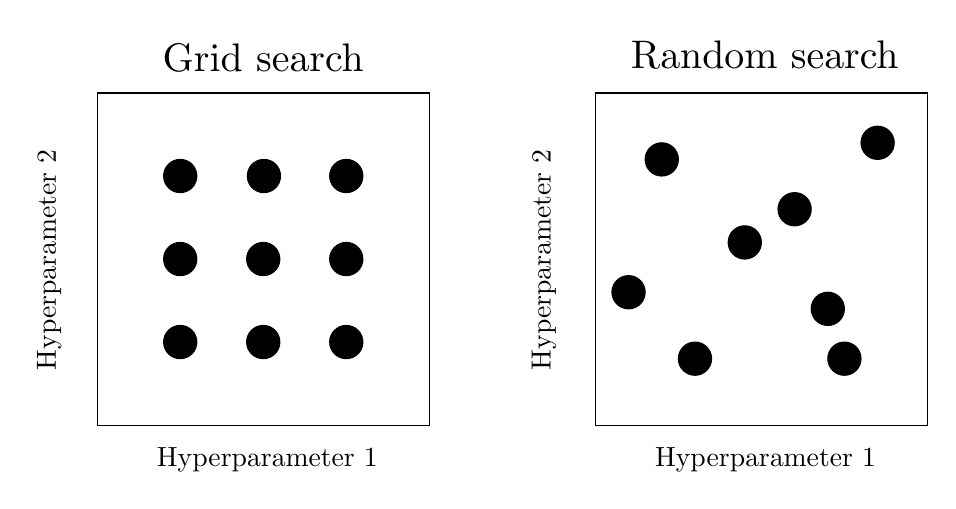
\begin{tikzpicture}[x=0.6pt,y=0.6pt,yscale=-1,xscale=1]
        %Shape: Rectangle [id:dp7765345595299928] 
        \draw   (40,40) -- (240,40) -- (240,240) -- (40,240) -- cycle ;
        %Shape: Rectangle [id:dp8266179045308344] 
        \draw   (340,40) -- (540,40) -- (540,240) -- (340,240) -- cycle ;
        %Shape: Circle [id:dp10989848309136652] 
        \draw  [fill={rgb, 255:red, 0; green, 0; blue, 0 }  ,fill opacity=1 ] (80,90) .. controls (80,84.48) and (84.48,80) .. (90,80) .. controls (95.52,80) and (100,84.48) .. (100,90) .. controls (100,95.52) and (95.52,100) .. (90,100) .. controls (84.48,100) and (80,95.52) .. (80,90) -- cycle ;
        %Shape: Circle [id:dp25798568532386523] 
        \draw  [fill={rgb, 255:red, 0; green, 0; blue, 0 }  ,fill opacity=1 ] (130.4,90) .. controls (130.4,84.48) and (134.88,80) .. (140.4,80) .. controls (145.92,80) and (150.4,84.48) .. (150.4,90) .. controls (150.4,95.52) and (145.92,100) .. (140.4,100) .. controls (134.88,100) and (130.4,95.52) .. (130.4,90) -- cycle ;
        %Shape: Circle [id:dp21802627978178712] 
        \draw  [fill={rgb, 255:red, 0; green, 0; blue, 0 }  ,fill opacity=1 ] (180,90) .. controls (180,84.48) and (184.48,80) .. (190,80) .. controls (195.52,80) and (200,84.48) .. (200,90) .. controls (200,95.52) and (195.52,100) .. (190,100) .. controls (184.48,100) and (180,95.52) .. (180,90) -- cycle ;
        %Shape: Circle [id:dp29856163256776613] 
        \draw  [fill={rgb, 255:red, 0; green, 0; blue, 0 }  ,fill opacity=1 ] (80,140) .. controls (80,134.48) and (84.48,130) .. (90,130) .. controls (95.52,130) and (100,134.48) .. (100,140) .. controls (100,145.52) and (95.52,150) .. (90,150) .. controls (84.48,150) and (80,145.52) .. (80,140) -- cycle ;
        %Shape: Circle [id:dp29841099273644034] 
        \draw  [fill={rgb, 255:red, 0; green, 0; blue, 0 }  ,fill opacity=1 ] (130,140) .. controls (130,134.48) and (134.48,130) .. (140,130) .. controls (145.52,130) and (150,134.48) .. (150,140) .. controls (150,145.52) and (145.52,150) .. (140,150) .. controls (134.48,150) and (130,145.52) .. (130,140) -- cycle ;
        %Shape: Circle [id:dp49228249173727456] 
        \draw  [fill={rgb, 255:red, 0; green, 0; blue, 0 }  ,fill opacity=1 ] (180,140) .. controls (180,134.48) and (184.48,130) .. (190,130) .. controls (195.52,130) and (200,134.48) .. (200,140) .. controls (200,145.52) and (195.52,150) .. (190,150) .. controls (184.48,150) and (180,145.52) .. (180,140) -- cycle ;
        %Shape: Circle [id:dp38157661859427416] 
        \draw  [fill={rgb, 255:red, 0; green, 0; blue, 0 }  ,fill opacity=1 ] (80,190) .. controls (80,184.48) and (84.48,180) .. (90,180) .. controls (95.52,180) and (100,184.48) .. (100,190) .. controls (100,195.52) and (95.52,200) .. (90,200) .. controls (84.48,200) and (80,195.52) .. (80,190) -- cycle ;
        %Shape: Circle [id:dp13924586669074634] 
        \draw  [fill={rgb, 255:red, 0; green, 0; blue, 0 }  ,fill opacity=1 ] (130,190) .. controls (130,184.48) and (134.48,180) .. (140,180) .. controls (145.52,180) and (150,184.48) .. (150,190) .. controls (150,195.52) and (145.52,200) .. (140,200) .. controls (134.48,200) and (130,195.52) .. (130,190) -- cycle ;
        %Shape: Circle [id:dp30928749690617674] 
        \draw  [fill={rgb, 255:red, 0; green, 0; blue, 0 }  ,fill opacity=1 ] (180,190) .. controls (180,184.48) and (184.48,180) .. (190,180) .. controls (195.52,180) and (200,184.48) .. (200,190) .. controls (200,195.52) and (195.52,200) .. (190,200) .. controls (184.48,200) and (180,195.52) .. (180,190) -- cycle ;
        %Shape: Circle [id:dp4482564100459898] 
        \draw  [fill={rgb, 255:red, 0; green, 0; blue, 0 }  ,fill opacity=1 ] (370,80) .. controls (370,74.48) and (374.48,70) .. (380,70) .. controls (385.52,70) and (390,74.48) .. (390,80) .. controls (390,85.52) and (385.52,90) .. (380,90) .. controls (374.48,90) and (370,85.52) .. (370,80) -- cycle ;
        %Shape: Circle [id:dp07124098077781627] 
        \draw  [fill={rgb, 255:red, 0; green, 0; blue, 0 }  ,fill opacity=1 ] (420,130) .. controls (420,124.48) and (424.48,120) .. (430,120) .. controls (435.52,120) and (440,124.48) .. (440,130) .. controls (440,135.52) and (435.52,140) .. (430,140) .. controls (424.48,140) and (420,135.52) .. (420,130) -- cycle ;
        %Shape: Circle [id:dp41745813324763004] 
        \draw  [fill={rgb, 255:red, 0; green, 0; blue, 0 }  ,fill opacity=1 ] (390,200) .. controls (390,194.48) and (394.48,190) .. (400,190) .. controls (405.52,190) and (410,194.48) .. (410,200) .. controls (410,205.52) and (405.52,210) .. (400,210) .. controls (394.48,210) and (390,205.52) .. (390,200) -- cycle ;
        %Shape: Circle [id:dp5867108869326927] 
        \draw  [fill={rgb, 255:red, 0; green, 0; blue, 0 }  ,fill opacity=1 ] (450,110) .. controls (450,104.48) and (454.48,100) .. (460,100) .. controls (465.52,100) and (470,104.48) .. (470,110) .. controls (470,115.52) and (465.52,120) .. (460,120) .. controls (454.48,120) and (450,115.52) .. (450,110) -- cycle ;
        %Shape: Circle [id:dp562496351098612] 
        \draw  [fill={rgb, 255:red, 0; green, 0; blue, 0 }  ,fill opacity=1 ] (480,200) .. controls (480,194.48) and (484.48,190) .. (490,190) .. controls (495.52,190) and (500,194.48) .. (500,200) .. controls (500,205.52) and (495.52,210) .. (490,210) .. controls (484.48,210) and (480,205.52) .. (480,200) -- cycle ;
        %Shape: Circle [id:dp7209986165291683] 
        \draw  [fill={rgb, 255:red, 0; green, 0; blue, 0 }  ,fill opacity=1 ] (470,170) .. controls (470,164.48) and (474.48,160) .. (480,160) .. controls (485.52,160) and (490,164.48) .. (490,170) .. controls (490,175.52) and (485.52,180) .. (480,180) .. controls (474.48,180) and (470,175.52) .. (470,170) -- cycle ;
        %Shape: Circle [id:dp586705666058086] 
        \draw  [fill={rgb, 255:red, 0; green, 0; blue, 0 }  ,fill opacity=1 ] (500,70) .. controls (500,64.48) and (504.48,60) .. (510,60) .. controls (515.52,60) and (520,64.48) .. (520,70) .. controls (520,75.52) and (515.52,80) .. (510,80) .. controls (504.48,80) and (500,75.52) .. (500,70) -- cycle ;
        %Shape: Circle [id:dp7017198962451507] 
        \draw  [fill={rgb, 255:red, 0; green, 0; blue, 0 }  ,fill opacity=1 ] (350,160) .. controls (350,154.48) and (354.48,150) .. (360,150) .. controls (365.52,150) and (370,154.48) .. (370,160) .. controls (370,165.52) and (365.52,170) .. (360,170) .. controls (354.48,170) and (350,165.52) .. (350,160) -- cycle ;
        
        % Text Node
        \draw (142.5,261) node  [align=left] {Hyperparameter 1};
        % Text Node
        \draw (442.5,261) node  [align=left] {Hyperparameter 1};
        % Text Node
        \draw (11,140.5) node [rotate=-270] [align=left] {Hyperparameter 2};
        % Text Node
        \draw (309,140.5) node [rotate=-270] [align=left] {Hyperparameter 2};
        % Text Node
        \draw (140,19) node [scale=1.44] [align=left] {Grid search};
        % Text Node
        \draw (442,17) node [scale=1.44] [align=left] {Random search};
    \end{tikzpicture}

    \caption{Grid and random search of nine trials. With grid search, nine trials only test three distinct values for each hyperparameter. On the other hand, with random search nien different values are explored for each hyperparameter. If one of these hyperparameters is much more important than the other (as is often the case) then random search is more likely to find promising regions of the space.}
    \label{grid_vs_random}
\end{figure}    
                
                \citeauthor{Bergstra} have shown empirically and theoretically that random search outperforms grid search using the same computational budget. They motivated these results suggesting that \textquote{random experiments are more efficient because not all hyperparameters are equally important to tune} and that \textquote{grid search experiments allocate too many trials to the exploration of dimensions that do not matter and suffer from poor coverage in dimensions that are important}. The authors also claim that it is easier to experiment with this technique:
                \begin{itemize}
                    \item Every trial can be carried out asynchronously.
                    \item The experiment can be stopped at any time and the trials carried out so far form a complete experiment.
                \end{itemize}
                See figure \ref{grid_vs_random} for a visual representation of grid search and random search.